%
% splines.tex
%
% (c) 2019 Prof Dr Andreas Müller, Hochschule Rapperswil
%
\section{Spline-Funktionen
\label{section:spline-funktionen}}
\rhead{Spline-Funktionen}
In diesem Abschnitt konstruieren wir ausgehend vom Haar-Wavelet mit Hilfe
der Faltung eine Familie $\varphi^{(n)}$ von Funktionen die zunehmend glatt
sind in dem Sinne, dass $\varphi^{(n)}$ für $n>1$ $n$ mal stetig
differenzierbar ist, und die alle eine Skalierungsrelation erfüllen.
Diese Funktionen werden wir dann im nächsten Abschnitt jeweils ein
Wavelet konstruieren.

\subsection{Das Haar-Wavelet
\label{subsection:spline:haar}}
Das Vaterwavelet des Haar-Wavelets war die charakteristische Funktion
des Einheitsintervalls
\begin{equation}
\varphi^{(0)}(t)
=
\chi_{[0,1)}(t)
=
\begin{cases}
1\qquad\qquad&0\le t < 1\\
0\qquad\qquad&\text{sonst}.
\end{cases}
\end{equation}
Aus $\varphi^{(0)}$ lässt sich wie in Kapitel~\ref{chapter:haar-wavelet}
ausgeführt eine Multiskalen-Analyse aufbauen.
Eine solche garantiert zunächst einmal eine lineare Darstellung von
$\varphi^{(0)}$ duch skalierte und translierte Kopien von $\varphi^{(0)}$
in der Form
\begin{equation}
\varphi^{(0)}(t)
=
\sqrt{2}
\sum_{k\in\mathbb Z}
h_k\varphi(2t-k)
=
\sum_{k\in\mathbb Z}
h_k D_{\frac12}T_k\varphi^{(0)}(t).
\label{splines:skalierungsrelation}
\end{equation}
Aus der Skalierungsrelation~\eqref{splines:skalierungsrelation}
kann man dann das Mutterwavelet gewinnen, wie in
Abschnitt~\ref{section:mutter-aus-vater} gezeigt wird.
Im Falle des Haar-Wavelets sind die Koeffzienten der
Skalierungsrelation
\[
\varphi^{(0)}(t)
=
\sqrt{2}
\biggl(
\frac1{\sqrt{2}}
\varphi^{(0)}(2t)
+
\frac1{\sqrt{2}}
\varphi^{(0)}(2t-1)
\biggr)
\qquad
\Rightarrow
\quad
h_0 = h_1 = \frac{1}{\sqrt{2}}.
\]
Nach Lemma~\ref{lemma:msa:psirelation} ist dann das Mutterwavelet
\[
\psi^{(0)}(t)
=
\sqrt{2}
\biggl(
\frac{1}{\sqrt{2}}
\varphi^{(0)}(2t)
-
\frac{1}{\sqrt{2}}
\varphi^{(0)}(2t-1)
\biggr),
\]
wie ebenfalls bereits in Kapitel~\ref{chapter:haar-wavelet} gezeigt wurde.
Auch wurde bereits auf die schlechten Stetikeitseigenschaften und
die schlechte Frequenz-Lokalisierung des Haar-Wavelets hingewiesen,
welche den praktischen Nutzen des Haar-Wavelets limitiert.
Damit stellt sich das Problem, ob man Funktionen gewinnen kann, die
eine ähnlich einfach zu gewinnende Skalierungsrelation haben,
aber bessere Lokalisierungseigenschaften im Frequenzbereich haben und
stetig oder sogar differenzierbar sind.

\subsection{Splines
\label{subsection:splines}}
Gesucht ist jetzt also eine Vaterwavelet-Funktion, welche ähnlich
einfach ist wie das eben in Erinnerung gerufene Haar-Wavelet, aber bessere 
Stetigkeitseigenschaften und damit bessere Lokalisierung im Frequenzbereich
hat.
Wir definieren die Funktionen $B_n=\varphi^{(n)}$ rekursiv wie folgt.

\begin{definition}
Die Funktion $\varphi^{(0)}$ ist wie vorhin die charakteristische Funktion
des Einheitsintervalls.
Für $n>0$ setzt man
\[
\varphi^{(n)} = \varphi^{(0)} * \varphi^{(n-1)}.
\]
Wir verwenden auch die Notation $B_n=\varphi^{(n)}$.
Die Funktionen $B_n(t)$ heissen $B$-Splines vom Grad $n$.
\end{definition}

Man beachte, dass die Funktionen $\varphi^{(n)}$ zwar in $L^2(\mathbb R)$ 
sind, aber sie sind nicht normiert.
Erst recht sind die Translate nicht orthonormiert, wie man das für eine
Multiskalenanalyse erwarten würde.

Explizit bedeutet die Definition der Funktion $\varphi^{(n)}$
\begin{equation}
\varphi^{(n)}(t)
=
\int_{-\infty}^\infty
\varphi^{(0)}(s)
\varphi^{(n-1)}(t-s)
\,ds
=
\int_0^1
\varphi^{(n-1)}(t-s)
\,ds
=
-
\int_t^{t-1}
\varphi^{(n-1)}(\tau)
\,d\tau
=
\int_{t-1}^t \varphi^{(n-1)}(\tau)\,d\tau
\label{eq:varphin-berechnung}
\end{equation}
mit der Substitution $\tau=t-s$.

\begin{lemma}
\label{lemma:phidiffbar}
Die Funktion $\varphi^{(n)}$ ist für $n>1$ $n$ mal stetig differenzierbar.
\end{lemma}

\begin{proof}[Beweis]
Mit Hilfe der Formel~\eqref{eq:varphin-berechnung} kann man die Ableitung
\begin{align*}
\frac{d}{dt}
\varphi^{(n)}(t)
&=
\frac{d}{dt} \int_{t-1}^t \varphi^{(n-1)}(\tau)\,d\tau
=
\varphi^{(n-1)}(\tau)\bigg|_{\tau=t}
-
\varphi^{(n-1)}(\tau)\bigg|_{\tau=t-1}
=
\varphi^{(n-1)}(t)-\varphi^{(n-1)}(t-1)
\end{align*}
berechnen.
Für $n>1$ ist die Funktion $\varphi^{(n-1)}$ stetig, also auch die
Ableitung.
Damit ist $\varphi^{(n)}$ einmal mehr differenzierbar als
$\varphi^{(n-1)}$.
Wiederholte Anwendung dieser Eigenschaft liefert die Aussage des Lemmas.
\end{proof}

\begin{beispiel}
Für $n=1$ finde man zum Beispiel
\[
\varphi^{(1)}(t)
=
\int_0^1 \varphi^{(0)}(t-s)\,ds
=
\begin{cases}
t\qquad\qquad&0\le t<1\\
2-t\qquad\qquad&1\le t<2\\
0\qquad\qquad&\text{sonst}
\end{cases}
\]
Die $L^2$-Norm davon ist
\[
\| \varphi^{(1)}\|^2
=
2
\int_0^1 t^2\,dt
=
2\biggl[\frac13t^3\biggr]_0^1
=
\frac23.
\]
Die Funktion $\varphi^{(1)}$ ist in Abbildung~\ref{spline:phi1}
dargestellt.
\begin{figure}
\centering
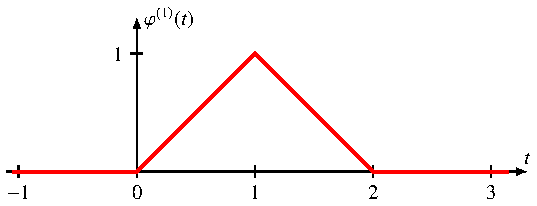
\includegraphics{chapters/9-spline/images/phi1.pdf}
\caption{Der Graph der Funktion $\varphi^{(1)}(t)$ zeigt, dass die
Funktion $\varphi^{(1)}$ stetig ist.
\label{spline:phi1}}
\end{figure}
\end{beispiel}

\begin{beispiel}
\begin{figure}
\centering
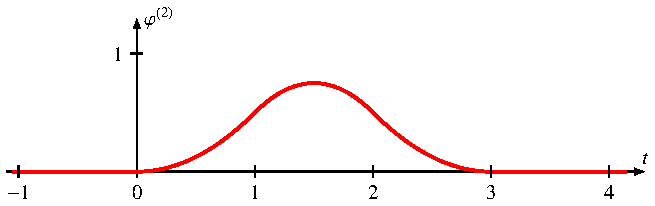
\includegraphics{chapters/9-spline/images/phi2.pdf}
\caption{Graph der Funktion $\varphi^{(2)}$
\label{spline:phi2}}
\end{figure}
Die Berechnung von $\varphi^{(2)}$ ist etwas aufwendiger.
Nach \eqref{eq:varphin-berechnung} muss
für $t\in\mathbb R$ das Integral von $\varphi^{(1)}$ über
das Intervall $[t-1,t]$ berechnet werden:
\begin{align*}
&t<0:
&
\varphi^{(2)}(t)
&=0
\\
0\le\,&t<1:
&
\varphi^{(2)}(t)
&=
\int_0^t\tau\,d\tau
=
\biggl[\frac12\tau^2\biggr]_0^t = \frac12t^2
\\
1\le\,&t<2:
&
\varphi^{(2)}(t)
&=
\int_{t-1}^1 \tau\,d\tau
+
\int_1^t 2-\tau\,d\tau
=
\biggl[\frac12\tau^2\biggr]_{t-1}^1
+
\biggl[2\tau-\frac12\tau^2\biggr]_1^t
%\\
%&&
%&=
%\frac12-\frac12(t-1)^2+2t-\frac12-\frac12t^2-2+\frac12
%\\
%&&
%&=
%\frac12-\frac12t^2+t-\frac12+2t-\frac12-\frac12t^2-2+\frac12
\\
&&
&=
-t^2+3t-\frac32
=
-\biggl(t-\frac32\biggr)^2+\frac34
\\
2\le\,&t<3:
&
\varphi^{(2)}(t)
&=
\int_{t-1}^2 2-\tau\,d\tau
=
\int_0^{3-t} s\,ds
=
\frac12(3-t)^2
\\
&t>3:
&
\varphi^{(2)}(t)
&=
0
\end{align*}
Der Graph der Funktion $\varphi^{(2)}$ ist in Abbildung~\ref{spline:phi2}
dargestellt.
In Übereinstimmung mit Lemma~\ref{lemma:phidiffbar} hat die Funktion
$\varphi^{(2)}$ keine offensichtlichen ``Knickpunkte''.
\end{beispiel}

\begin{beispiel}
\begin{figure}
\centering
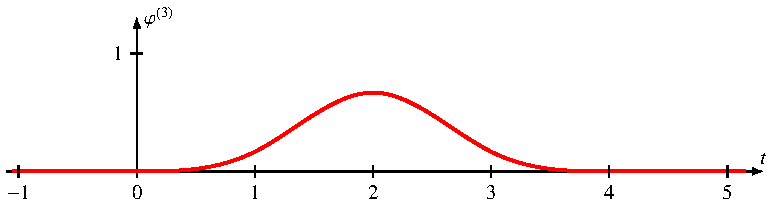
\includegraphics{chapters/9-spline/images/phi3.pdf}
\caption{Graph der Funktion $\varphi^{(3)}$.
\label{spline:phi3}}
\end{figure}
Für $\varphi^{(3)}(t)$ stellen wir nur die Resultate
zusammen, die leicht mit Hilfe eines Computer-Algebra-Systems
gewonnen werden können:
\begin{equation}
\varphi^{(3)}(t)
=
\begin{cases}
\displaystyle
\phantom{-}
\frac16t^3
&\qquad
0\le t<1
\\[9pt]
\displaystyle
-\frac12t^3+2t^2-2t+\frac23
&\qquad
1\le t<2
\\[9pt]
\displaystyle
\phantom{-}
\frac12t^3-4t^2+10t-\frac{22}3
&\qquad
2\le t<3
\\[9pt]
\displaystyle
-\frac16(t-4)^3
&\qquad
3\le t<4
\\[9pt]
\displaystyle
\phantom{-}
0&\qquad\text{sonst}
\end{cases}
\label{phi3-polynome}
\end{equation}
Der Graph der Funktion $\varphi^{(3)}$ ist in Abbildung~\ref{spline:phi3}
dargestellt.
\end{beispiel}

Aus den Beispielen kann man ablesen, dass die Funktionen
$B_n(t)=\varphi^{(n)}(t)$ auf jedem Intervall der Form $[k,k+1)$ 
ein Polynom vom Grad $n$ ist.
Wir sagen, $B_n$ sei stückweise {\em Grad-$n$-polynomiell}.
\index{Grad $n$-polynomiell}
Man kann zeigen, dass die vier Polynome auf der rechten
Seite von~\eqref{phi3-polynome} linear unabhängig sind.
Wir vermuten, dass die Translate von $B_n$ auf jedem Intervall der Form
$[k,k+1)$ {\em linear unabhängige} Polynome vom Grad $n$ sind.
Dies bedeutet, dass durch Linearkombination von Translaten der
Funktionen $B_n$ jede beliebige stückweise Grad-$n$-polynomielle
Funktion dargestellt werden kann.
Die Funktionen $B_n$ bilden somit eine Basis des Raums der stückweise 
Grad-$n$-polynomiellen Funktionen.
Dies erklärt die Bedeutung der Funktionen $B_n$ in der Numerik.
Besonders die Funktionen $B_3$ spielen eine grosse Rolle in den
Anwendungen.
Zum Beispiel werden solche kubischen Splines für die Beschreibung
von Kurven in der Computergraphik verwendet.

\subsection{Skalierungsrelation für $\varphi^{(n)}$
\label{subsection:skalierungsrelation-phin}}
Die Funktionen $B_n=\varphi^{(n)}$ können nur dann Anlass zu einer
Multiskalen-Analyse geben, wenn sie die Skalierungseigenschaft
besitzen.
Wir wissen bereits aus Abschnitt~\ref{subsection:spline:haar},
dass das Haar-Wavelet $\varphi^{(0)}$ die Skalierungsrelation
mit den Koeffizienten $1/\sqrt{2}$ erfüllt.
Satz~\ref{satz:faltung-linearkombination} garantiert, dass mit
$\varphi^{(n-1)}$ auch $\varphi^{(n)}$ die Skalierungseigenschaft hat.
Wir haben in~\eqref{eq:faltung-linearkombination}
sogar eine Formel, mit der wir die Koeffizienten der Skalierungsrelation
berechnen können.

\begin{beispiel}
Wir bestimmen die Koeffizienten der Skalierungsrelation von $\varphi^{(1)}$.
Da $\varphi^{(1)}=\varphi^{(0)}*\varphi^{(0)}$ folgt mit den bekannten
Koeffizienten $\varphi^{(0)}_0=\varphi^{(0)}_1=1/\sqrt{2}$ die
Formel~\eqref{eq:faltung-linearkombination}
\[
\begin{aligned}
\varphi^{(1)}_0
&=
\frac1{\sqrt{2}}
\varphi^{(0)}_0
\cdot
\varphi^{(0)}_0
&&=
\frac{1}{2\sqrt{2}}
=\frac{1}{2\sqrt{2}}\binom{2}{0}
\\
\varphi^{(1)}_1
&=
\frac1{\sqrt{2}}
(
\varphi^{(0)}_0
\cdot
\varphi^{(0)}_1
+
\varphi^{(0)}_1
\cdot
\varphi^{(0)}_0
)
&&=
\frac{2}{2\sqrt{2}}
=\frac{1}{2\sqrt{2}}\binom{2}{1}
\\
\varphi^{(1)}_2
&=
\frac1{\sqrt{2}}
\varphi^{(0)}_1
\cdot
\varphi^{(0)}_1
&&=
\frac{1}{2\sqrt{2}}
=\frac{1}{2\sqrt{2}}\binom{2}{2}
\end{aligned}
\]
Diese Koeffizienten haben wir im Wesentlichen schon in
\eqref{eq:skalierung-phi1-proto} angetroffen.
Das Auftauchen von Binomialkoeffizienten auf der rechten Seite wird
durch den nachfolgenden Satz~\ref{spline:satz:koef} erklärt.
\end{beispiel}

Das Beispiel lässt sich verallgemeinern und führt auf den folgenden Satz.

\begin{satz}
\label{spline:satz:koef}
Die Funktion $\varphi^{(n)}$ hat die Skalierungseigenschaft  mit den
Koeffizienten
\[
\varphi^{(n)}_k = \frac{\sqrt{2}}{2^{n+1}}\binom{n+1}{k}.
\]
für $0\le k\le n$.
\end{satz}
Die zugehörige erzeugende Funktion Funktion ist
\begin{equation}
\tilde{H}_n(\omega)
=
\frac{1}{\sqrt{2}}
\sum_{k=0}^{n+1}
\varphi_k^{(n)} e^{-ik\omega}
=
\frac{1}{\sqrt{2}}
\sum_{k=0}^{n+1}
\frac{\sqrt{2}}{2^{n+1}}
\binom{n+1}{k}
e^{-ik\omega}
=
\sum_{k=0}^{n+1}
\frac{1}{2^{n+1}}
\binom{n+1}{k}
e^{ik\omega}
=
\biggl(
\frac{1+e^{-i\omega}}{2}
\biggr)^{n+1},
\end{equation}
wir werden sie in Abschnitt~\ref{subsection:spline-ft} verwenden,
um die erzeugende Funktion für die orthonormalisierten Spline-Wavelets
zu berechnen.


